\section{Introduzione}\label{Introduzione}
Il modello di Ising è un sistema statistico che si propone di modellizzare un mezzo continuo ferromagnetico.

L'idea di base è simile al principio fondamentale della termodinamica statistica dei mezzi continui (come i gas perfetti ad esempio), tale per cui si amette che le proprietà macroscopiche di un materiale siano manifestazione di una struttura microscopica corpuscolare.

\begin{wrapfigure}{r}{0.4\textwidth}
\vspace{-30pt}
  \begin{center}
      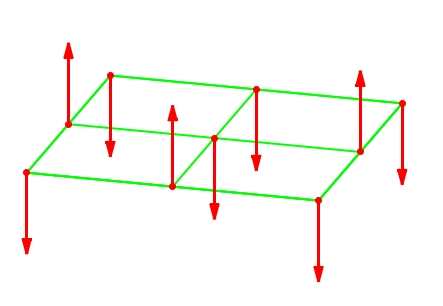
\includegraphics[scale=0.45]{Immagini/Isingmodel.jpg}
  \end{center}
\vspace{-20pt}
  \caption{Modello di Ising: Ogni punto macroscopico contiene un reticolo di Spin.}\label{fig:1}
\vspace{-10pt}
\end{wrapfigure}
In questa ottica è possibile parlare di \emph{punto macroscopico} visto come una scatola, di dimensioni trascurabili (quindi puntiforme) rispetto alla scala caratteristica del corpo, al cui interno sia contenuto un sistema microscopico semplice costituito da un numero statisticamento significativo di punti materiali.

Pertanto le proprietà macroscopiche del corpo continuo( per esempio temperatura, pressione, magnetizzazione) misurate in un punto dipendono dallo stato microscopico del sistema statistico contenuto nel punto macroscopico.
Mentre nel caso del continuo gassoso si modellizza il sistema microscopico come un numero grande di punti materiali sottoposti alle leggi della meccanica classica, per il continuo ferromagnetico il modello del sistema microscopico è , appunto, quello di Ising.

\paragraph{Proprietà del modello}

\begin{itemize}
\item Il modello di Ising è un sistema costituito da una collezione di $N$ (numero costante e "grande", tendente ad $\inf$ nel limite termodinamico) dipoli magnetici $s_{i}$ posti ai vertici (indicizzati $i$) di un reticolo n-dimensionale di forma quadrata ($n=3$ nello spazio fisico).
D'ora in poi si indicherà con $l$ il passo del reticolo (costante dimensionale) perciò il lato del reticolo risulterà pari ad $L = l n$ dove $n$ indica il numero di spin in una riga, nel limite termodinamico $l\rightarrow 0$ e il reticolo tende al continuo.

\item Il modello è un sistema statistico, i valori degli spin per ogni nodo costituiscono le variabili aleatorie e i possibili valori che assunti sono determinati in accordo con i principi della meccanica quantistica. Pertanto la componente di ogni spin lungo lo stesso asse prescelto può assumere solo due valori\footnote{ In una sostanza ferromagnetica vera ci si aspetterebbe che i dipoli fondamentali che la costituiscano possano assumere ogni direzione nello spazio. In questo caso ci si limita ad una sola componente in prospettiva di considerare il corpo immerso in una campo magnetico esterno (considerato uniforme nel volume del punto macroscopico dove vive il sistema di ising microscopico) che fornisce una direzione privilegiata lungo cui considerare l'orientazione dei domìni magnetici.} 
$$s_{i}\in \lbrace \pm 1 \rbrace$$
e non è possibile determinare le componenti su più assi contemporaneamente.
In questo caso lo spazio delle configurazioni $\Gamma$ del sistema ha cardinalità $2^{N}$.

\item Gli Spin interagiscono con il campo esterno e tra di loro ma tale interazione reciproca avviene solo tra spin primi vicini. Risulta che l'energia di uno specifico stato $\sigma =\lbrace\ldots , s_{i} ,\ldots \rbrace$ è data dalla Hamiltoniana:
\begin{equation}\label{Hamiltoniana}
H = - J \sum_{<i,j>}s_{i}s_{j}  -B\sum_i s_i
\end{equation}
dove $J$ è la costante dimensionale dell' energia di interazione e $B$ è l'intensità del campo magnetico esterno.

\item Il sistema modellizza un punto macroscopico quindi lo si pensa circondato da altri sistemi dello stesso tipo, siccome l'interazione avviene solo tra primi vicini il sistema preso in considerazione sarà interessato solo dai reticoli immediatamente adiacenti.
\begin{figure}[h!]
\centering
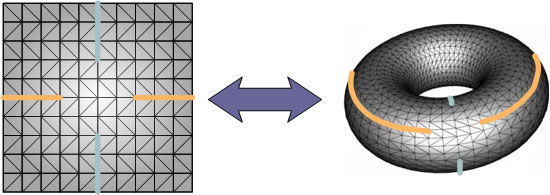
\includegraphics[scale=0.5]{Immagini/bordoperiodico.jpg}
\caption{Condizione di Bordo periodico: reticolo Toroidale.}\label{fig:2}
\end{figure}
Ammettendo che il sistema possa essere considerato continuo, i reticoli adiacenti saranno da considerare infinitamente vicini in scala macroscopica. 
Se il sistema macroscopico soddisfa la condizione di equilibrio termico si avrà necessariamente che due punti macroscopici infinitamente vicini si troveranno in uno stato tendenzialmente simile a quello del sistema sotto esame.
Per approssimare questa caratteristica si può assumere che singolo sistema studiato sia circondato da copie oppure, equivalentemente, che il reticolo soddisfi al condizione di bordo periodico.

\end{itemize}
\bigskip
Nell'ambito della meccanica statistica si rinuncia alla descrizione deterministica della dinamica del sistema microscopico (per quanto i suoi costituenti siano semplici essi sono in un numero troppo grande) e si è interessati a determinarne solo le proprietà colletive ( o macroscopiche se si interpreta l'intero sistema come un punto).
Di conseguenza il singolo stato microscopico perde di rilevanza, ciò che conta sono gli \emph{Ensamble Statistici} ovvero la coppia $\xi = (A_{\xi},\rho)$ costituita da $A\subseteq \Gamma$, collezioni di tutte le configurazioni microscopiche che il sistema può effettivamente occupare, e da $\rho:\Gamma \rightarrow \mathbb{R}$ distribuzione di probabilità degli specifici stati microscopici in cui il sistema può trovarsi.

In questo ambito gli ensemble statistici assumono il ruolo che avevano le \emph{configurazioni} per  un sistema meccanico classico mentre il ruolo di \emph{coordinate di configurazione} è ora svolto dalle variabili termodinamiche (dette anche variabili di stato) come ad esempio la temperatura, il volume, e la densità . 
Quindi le variabili di stato fissano l'ensemble (stato macroscopico) e la probabilità che il sistema si trovi nello stato microscopico $\sigma \in \Gamma$ sarà data $\rho(\sigma)$ (se $\Gamma$ è discreto il valore è definito nella singola configurazione).
\medskip

Il modello di Ising appena descritto è un sistema isolato (il campo uniforme B esterno è da considerarsi come un parametro fisso del sistema) in equilibrio termico con la riserva di di calore del sistema ambiente.
Lo stato "macroscopico" per sistemi che scambiano energia solo sotto forma di calore mantenendo volume e numero di elementi costante (il reticolo rimane immutato evolvono solo i versi degli spin) è dato dagli \emph{ensemble canonici}. 
Ensemble di questo tipo sono caratterizzati da un'unica variabile di stato, la temperatura T, l'insieme $$\xi = \xi(T)$$ che li costituisce coincide sempre con l'intero spazio delle fasi 
$$A_{\xi}\equiv \Gamma$$
e la funzione di probabilità ad essi associato è data dalla distribuzione di Boltzmann
$$\rho(\phi) = \frac{e^{-\beta H(\phi)}}{Z} $$
con $\phi \in A\equiv \Gamma$ generico microstato, $\beta = \frac{1}{k_{B}T} $( $k_B$ è la costante di Boltzman) e con $Z$ funzione di partizione: 

\begin{equation}\label{Partizione}
Z = \int_{\Gamma} \textsf{D}\phi \, e^{-\beta H(\phi)}
\end{equation}
($\textsf{D}\phi$ è la misura sullo spazio $\Gamma$, quando $\Gamma$ è finito l'integrale si riduce ad una sommatoria su tutti gli stati).


\subsection{Metodi Numerici}

Come in ogni altro caso, per poter implementare il calcolo al computer è necessario ridurre tutti i parametri a quantità adimensionali. D'ora in poi tutte le costanti dimensionali saranno poste unitarie:
$$ k_B = 1 \qquad J=1$$
inoltre verrà trascurata l'interazione del campo magnetico esterno $B=0$ e ci si limiterà al modello di Ising bidimensionale $D=2$.
\newline
Con tali convenzioni la variabile $\beta$ equivarrà semplicemente alla temperatura inversa $\beta= \dfrac{1}{t}$.
\medskip

Per studiare il comportamento del sistema termalizzato a seconda della temperatura è necessario analizzare l'andamento dei valori d'aspettazione delle osservabili macroscopiche del sistema.
In generale per calcolare i valori di aspettazione è necessario calcolare integrali sullo spazio delle fasi, per esempio il valore d'aspettazione $O$ (dove $O(\phi)$ è il valore definito sul singolo microstato) risulta: 
\begin{equation}\label{aspettazione teo}
\langle O \rangle = \frac{\int_{\Gamma} \textsf{D}\phi \,O(\phi) e^{-\beta H(\phi)}}{Z}
\end{equation}

Il calcolo computazionale di questo oggetto è proponibile solo limitandosi a sistemi di Ising con $N$ finito. In questo caso risulterebbe:
\begin{equation}\label{aspettazione finito}
\langle O \rangle = \frac{\sum_{n=0}^{N} O_n e^{-\beta E_n}}{\sum_{n=0}^{N} e^{-\beta E_n}}
\end{equation}
con $O_n$ e $H_n$ valori degli osservabili sullo stato $\phi_n$.

Quest'equazione dimostra come sia possibile calcolare esattamente $\langle O \rangle$ per modelli con $N$ finito anche a livello computazionale. Teoricamente basterebbe generare tutti i possibili stati, pesarli con il loro peso di Boltzman relativo alla temperatura $T$ che si intende studiare e sommarli secondo la formula.
Siccome ci si pone l'obbiettivo  di estrapolare la teoria del sistema di Ising completo (quindi al limite termodinamico) sarà necessario simulare il sistema per dei numeri di spin sufficientemente alti.
Per questo il metodo esatto si dimostra inutilizzabile per due motivi: 
\begin{enumerate}
\item estremamente lungo: bisogna simulare $2^{n_{riga}^D}$ stati
\item estremamente inefficiente: la maggior parte del tempo macchina viene sprecato per generare configurazione di peso trascurabile, infatti le configurazioni con energia "lontana"(a seconda della temperatura) dal valore medio contribuiscono in modo irrilevante al valare d'aspettazione.
\end{enumerate}
Per questo motivo sarà necessario avvalersi dei metodi approssimati di \emph{Montecarlo}.

\subsubsection{Calcolo della funzione di Partizione: Importance Sampling}
Alla base dei metodi Montecarlo c'è l'idea di non generare tutto lo spazio degli stati ma campionare solo alcune configurazioni scelte in modo (pseudo-)casuale in numero statisticamente significativo.
Naturalmente se si procedesse a generare stati con una distrubuzione di probabilità uniforme si incorrerebbe esattamente negli stessi problemi di prima, infatti in tal caso sarebbero comunque necessari un numero di stati campione paragonabile alla cardinalità di $\Gamma$  per ottenere una stima affidabile.

La soluzione ideale è sfruttare il metodo dell'\emph{Importance Sampling} secondo cui gli stati non vengono generati in modo uniforme ma secondo la distribuzione attesa di Boltzman. In questo modo la collezione di configurazioni raccolta conterrà gli stati più pesanti con maggiore probabilità rispetto agli altri.
Risulta che se $\lbrace\phi_i\rbrace _{0\leq i \leq K}$ sono degli stati generati in modo casuale secondo la distribuzione di Boltzman il valore medio di questi valori è una buona stima del valore di aspettazione, ovvero:
\begin{equation}\label{aspettazione Monte}
\sum_{i=1}^K O(\phi_i) \xrightarrow[K\rightarrow \infty]{} \langle O \rangle
\end{equation}

Il problema che rimane aperto è in che modo generare una sequenza di configurazioni in accordo con la distribuzione di probabilità richiesta e che quindi generi gli stati più probabili con frequenza maggiore rispetto agli altri.
Per questo si introducono le \emph{Catene di Markov Montecarlo}.

\subsubsection{Catena di Markov MonteCarlo} 
Una \emph{Catena di Markov} in $\Gamma$ è una sequenza di configurazioni $(X_0, X_1\ldots)$ completamente definita da una \emph{Matrice di transizione di probabilità} $P: \Gamma \rightarrow \Gamma$ che a partire dallo stato $X_l$ determina l'elemento successivo della successione $X_{(l+1)}$ in modo totalmente indipendementente dagli altri elementi  $X_i$ con $i<l$ precedenti.
\newline
La catena costruita a partire da un elemento scelto non è univoca, infatti gli elementi della matrice $[P]_{ij}$ rappresentano la probabilità di avere una transizione dallo stato $i$ allo stato $j$ e in generale tale probabilità sarà diversa da $0$ per una grande varietà di configurazioni in $\Gamma$.
\newline
Vale il seguente teorema:
\begin{thm}\label{teorema markov}$\\$%\begin{thm}[nome teorema]
HP:	Si consideri una catena di Markov $(X_0, X_1\ldots)$ di matrice di transizione $P$tale che:\begin{itemize}
	\item[-] P sia \emph{irriducibile}, ovvero: $\quad \forall X_i, X_j \in \Gamma \quad \exists n\in \mathbb{N}\quad | \quad [P^n]_{ij}>0$
	\item[-] $(X_0, X_1\ldots)$ sia \emph{aperiodica}, ovvero: $\quad \forall X_i \quad [P]_{ii}>0$
	\end{itemize}
$\\$ Te: $$\forall i,j \qquad \exists 1! \lim_{n\rightarrow \infty}[P^n]_{ij} = \pi(j) \quad | \quad \sum_{j\in \Gamma} \pi(j) = 1$$
\end{thm} 

In sostanza l'applicazione di una matrice di transizione, costruita in modo da rendere accessibile qualsiasi altro stato con probabilità non nulla, ripetuta un numero $n$ di volte (tendente all'infinito) ad uno stato $X_0$ determina un unica distribuzione di probabilità dei possibili stati finali, $\pi(i_{fin})$ detta \emph{distribuzione d'equilibrio}, qualsiasi sia lo stato iniziale scelto.
\bigskip \newline
Tutto ciò conduce ad una criterio per risolvere il problema posto nel paragrafo precedente, se:
\begin{itemize}

\item Viene costruito un operatore $P: \Gamma \rightarrow \Gamma$ tale da mandare uno stato del sistema di Ising in un altro stato scelto in modo pseudo-casuale ma sempre in accordo con i valori della matrice di probabilità di transizione.
 
\item La matrice di transizione relativa a $P$ soddisfa il teorema precedente ed è tale per cui la sua distribuzione di equilibrio concida con la distribuzio di Boltzman prevista al valore di temperatura inversa $\beta$ fissato .

\item Tale operatore viene applicato ad un qualsiasi stato iniziale $X_i \in \Gamma$ un numero $n_{eq}$ di volte sufficiente a termalizzare il sistema, ovvero tale che la probabilità di transizione da $X_i$ ad $X_f$ risulti simile a quella d'equilibrio (ad esempio $n_eq$ può essere considerato sufficiente grande quando   $[P^{n_{eq}}]_{ij} \simeq [P^{n_{eq}+1}]_{ij}$).

\item[$\triangleright$] \underline{Allora} tutti gli stati ottenuti dalle successive applicazioni dell'algoritmo $P$ costituiranno una catena di Markov $(X_{(n_eq + 1)}, X_{(n_eq + 2)}, \ldots, X_{(n_eq + K)}$ che rappresenta un'ottima approssimazione di una raccolta statistica di configurazioni casuali con distribuzione di Boltzman a $beta$ fissato.\newline
Si parla in questo caso di \emph{Catene Markov - Montecarlo}.

\end{itemize} 

Questa approccio ha un' interpretazione fisica intuitiva: l'algoritmo $P$ cerca di simulare l'evoluzione temporale del sistema statistico che, non essendo deterministica, sarà soggetta a continue fluttuazioni termiche.
La termalizzazione sarà l'equivalente del tempo richiesto ad un corpo materiale di raggiungere la temperatura dello spazio ambiente. 
Il Valore d'aspettazione di un osservabile sul sistema sarà quindi da interpretare come media temporale su tutti gli stati occupati dal sistema nella sua evoluzione "caotica" in accordo con l'equazione \ref{aspettazione Monte}. In questo senso l'algoritmo scelto per realizzare l'operatore $P$ determina e simula la dinamica del sistema statistico.
\medskip\newline
Esistono diversi algoritmi che realizzano questo metodo di Markov-Montecarlo che si differenziano per il modo con cui viene realizzato l'operatore di evoluzione $P$. In questo articolo ne verranno implementati due: l'algoritmo di \emph{Metropolis} e l'algoritmo di \emph{Swenden-Wang}\footnote{ La dimostrazione che le matrici di probabilità di transizione relative a questi algoritmi soddisfino le ipotesi del teorema \ref{teorema markov} desiderate si può trovare in \cite{Newman2001}.} .

\paragraph{Algoritmo di Metropolis}
In questo caso l'operatore \emph{"step di evoluzione"} $P$ viene ottenuto ripetendo il seguente algoritmo almeno una volta per ogni spin del reticolo (il modo più semplice per farlo e passare in rassegna in modo sequenziale tutti i nodi):
\bigskip

\begin{tikzpicture}[node distance = 2cm, auto]
    % Place nodes
    \node [block] (init) {Scegliere un nodo $i$ sul reticolo. \newline \footnotesize(Sarà necessario scansionarli tutti in modo sequenziali almeno una volta)};
    \node [block, below of=init,node distance=3.cm] (flip1) {Flip del nodo $i$.  \small \newline $E \longmapsto E - 2\cdot E_i$\newline $S \longmapsto S - 2\cdot\sigma_i$};
    \node [decision, below of=flip1,node distance=3.cm] (test1) {$\Delta E = - 2 E_i > 0$ ?};
    \node [block, right of=test1, node distance=6.15cm] (accetto) {La proposta di Flip è accettata.};
	\node [block, left of=test1, node distance=6.15cm] (rifiuto) {La proposta di Flip è rifiutata. \newline\footnotesize( Flip del nodo $i$ per tornare alla configurazione inziale)};
	\node [block, below of=test1,node distance=3.cm] (preparazione) {La nuova configurazione è da accettare con probabilità $P = e^{- 2 \beta \Delta E}$. \newline \footnotesize (Si Genera un numero pseudorandom $0<r<1$ con distribuzione uniforme.) };
    \node [decision, below of=preparazione] (test2) {$r<e^{- 2 \beta \Delta E}$ ?};

    % Draw edges
    \path [line] (init) -- (flip1);
    \path [line] (flip1) -- (test1);
    \path [line] (test1) -- node [near start] {No} (accetto);
    \path [line] (test1) -- node {Sì}(preparazione);
    \path [line] (preparazione) -- (test2);
    \path [line] (test2) -| node [near start] {No} (rifiuto);
    \path [line] (test2) -| node [near end]{Sì}(accetto);
    \path [line] (rifiuto) |- (init);
    \path [line] (accetto) |- (init);
\end{tikzpicture}
\medskip\newline
L'algoritmo di Metropolis prevede che una configurazione evolva naturalmente ad una configurazione ad energia minore( test 1) ma non esclude le fluttuazioni termiche, infatti il sistema può fluttuare in configurazioni ad energia più elevata con una probabilità che dipende dalla temperatura dell'ambiente in cui è immerso il sistema (test 2).


\paragraph{Algoritmo di Swenden-Wang}
L'algoritmo di Swenden-Wang prevede due fasi:
\begin{enumerate}
\item Si suddivide il sistema in Cluster, sottoinsiemi di spin paralleli limitrofi.
\item Ogni cluster viene invertito con probabilità $1/2$.
\end{enumerate}
\medskip Resta da stabilire il criterio con cui vengono costruiti i cluster:
\newline
Due nodi primi vicini appartegono allo stesso cluster se solo se fra di loro si costituisce un legame (bond attivato). L'attivazione di un bond tra due spin limitrofi è un evento statistico che avviene con probabilità
\begin{equation}
P_{bond}(i,j) = \begin{cases}
				0 & \textit{se } \sigma_i \neq \sigma_j \\
				1 - e^{-2\beta} & \textit{se } \sigma_i \neq \sigma_j \\
				\end{cases}
\end{equation}
\medskip Dalle caratteristiche dei cluster è possibile ricavare delle stime di alcune osservabili sul sistema:
\begin{enumerate}
\item la magnetizzazione assoluta $|M|= |\sum_{i=0}^{N}\dfrac{\sigma_i}{N}|$ corrisponde alla taglia massima del cluster più grande (rapporto tra numero di elementi del cluster e numero di elementi totali).
\item il quadrato della magnetizzazione assoluta $M^2$ corrisponde alla media dei quadrati delle taglie di tutti i cluster formati.
\end{enumerate}


\subsection{Implementazione Computazionale}
Per simulare il sistema di Ising implementando gli algoritmi precedenti è stato utilizzato il linguaggio \C++. 
\newline
Il cuore della simulazione è la classe "microstato" che rappresenta la configurazione microscopica del sistema di Ising.
L'attributo principale è l'array bidimensionale \texttt{StatoSpin} di tipo \texttt{int} che contiene le orientazioni di ogni singolo spin arrangiandoli in una matrice $\sigma_{i\, j}$.
\begin{center}
\begin{tabular}{ c c c c c c} 
 			 & $\vdots$ 			   & 			 & $\vdots$ 				&    & \\ 
 			 & $|$ 			   & 			 & $|$ 				&    & \\ 
 \textemdash & $\sigma_{1\,0}$ & \textemdash & $\sigma_{1\,1}$  & \textemdash & $\cdots$   \\
  			 & $|$ 			   & 			 & $|$ 				&   & \\ 
 \textemdash & $\sigma_{0\,0}$ & \textemdash & $\sigma_{0\,1}$  & \textemdash & $\cdots$  \\ 
 			 & $|$ 			   & 			 & $|$ 				&   &  \\ 
\end{tabular}
\end{center}
La classe contiene i prototipi di "evoluzione", metodi che a partire da un valore dato di $\beta$, trasformano il microstato (aggiornando la matrice $\sigma_{i\,j}$) nella configurazione a lui successiva nella catena di Markov-Montecarlo, chiaramente sarà definito un metodo diverso per ogni algoritmo preso in considerazione (Metropolis e Swenden-Wang).
I metodi di "raccolta" invece applicano consecutivamente i metodi di evoluzione e ad ogni passo raccolgono il valore delle osservabili microscopiche necessarie per stimare i valori d'aspettazione d'ensemble.
\newline \medskip
La struttura del codice è la seguente
\tikzstyle{every node}=[draw=black,thick,anchor=west]
\tikzstyle{selected}=[draw=red,fill=red!30]
\tikzstyle{optional}=[dashed,fill=gray!50]

\begin{tikzpicture}[%
  grow via three points={one child at (0.5,-0.7) and
  two children at (0.5,-0.7) and (0.5,-1.4)},
  edge from parent path={(\tikzparentnode.south) |- (\tikzchildnode.west)}]
  \node [casella] {\emph{microstato.struttura.h}

    }
    child { node [casella] {\emph{Controllo.h}}}		
    child { node [casella] {evoluzione}
      child { node [casella] {\emph{Metropolis.h}}}
      child { node [casella] {\emph{Multiclusterclass.h}}}
    }			
    child [missing] {}				
    child [missing] {}				
    child { node {\emph{Raccolta.h}}};
   
\end{tikzpicture}

Questi file costituiscono l'\emph{header} che è stato incluso nei codici utilizzati per generare i grafici mostrati nei capitoli successivi. 
Le sorgenti di tali file si avvarrano anche di ulteriori header contenenti delle funzioni utili per analizzare i dati ricavati dalla simulazione:
\begin{itemize}
\item \emph{funzioni\_utili.h} per generare file di dati compatibili con "Gnuplot"
\item \emph{funzioni\_statistica.h} per l'analisi statistica dei dati e il calcolo degli errori sui valori d'aspettazione.
\end{itemize}

\subsubsection*{Metodo di evoluzione a Multicluster}
La suddivisione del sistema in cluster è l'operazione più impegnativa della simulazione. Per eseguirla viene introdotta una classe ausiliaria \texttt{Cluster} i cui attributi sono la lista dei nodi appartenti al cluster, il numero di elementi e un etichetta (label).
La classe possiede un metodo di somma che permette di aggregare due cluster in uno solo, conservando un unico label e unendo le due liste di elementi.
L'implementazione avviene nel seguente modo:
\begin{enumerate}
\item Ad ogni nodo viene attribuito un proprio label e una variabile cluster. Inolte viene costruita una lista dei gli interi effettivamente utilizzati come label di qualche cluster del sistema.
\item Si passano in rassegna tutti i nodi per verificare se il bond con lo spin primo vicino a destra viene attivo (ricordando la convenzione di bordo periodico).\newline
In caso affermativo l'etichetta del nodo a destra viene eliminata dalla lista dei label effettivi e si uniscono i cluster relativi ai label della coppia di nodi presi in considerazione. L'unione prevede che tutti i nodi appartenenti allo stesso cluster abbiano alla fine lo stesso label.
\item Si passano in rassegna tutti i nodi testando questa volta i bond in verticale.
\item A questo punto la lista dei labelli effettivi permette di scorrere tra tutte le variabili cluster che contengono nella loro lista almeno uno spin del sistema (e che complessivamente suddividono il reticolo). In questo modo è possibile invertire i  singoli cluster ed estrarre informazioni su di essi.
\end{enumerate}